%\section{Практична реалізація}
\section{ПРАКТИЧНА РЕАЛІЗАЦІЯ}

Даний розділ присвячується аналізу часового ряду тестувальної системи DOTS за допомогою мови програмування Python. 

Python $-$ це легка в освоєнні, потужна мова програмування. Він має ефективні структури даних високого рівня і простий, але ефективний підхід до об'єктно-орієнтованого програмування [7].

Python став загальноприйнятою мовою програмування для багатьох сфер застосування науки про дані. Дана мова програмування поєднує в собі міць мов програмування з простотою використання предметно орієнтованих скриптових мов типу MATLAB або R. 

В Python є бібліотеки для завантаження даних, візуалізації, статистичних обчислень, обробки природної мови, обробки зображень і багато чого іншого [8].

Також використовувався фреймфорк Anaconda. Це безкоштовний, включаючи комерційне використання, і готовий до використання в середовищі підприємства дистрибутив Python, який об'єднує всі ключові бібліотеки Python, необхідні для роботи в області науки про дані, математики та розробки, в одному зручному для користувача крос-платформенном дистрибутиві [9].

Для тренування нейронних мереж було обрано бібліотеку PyTorch. PyTorch - це бібліотека для програм Python, яка сприяє побудові проектів глибокого навчання [10].

Також використовувалась бібліотеки NumPy та matplotlib. NumPy є основним пакетом для наукових обчислень з Python [11]. Matplotlib $-$ це всебічна бібліотека для створення статичних, анімованих та інтерактивних візуалізацій у Python [12]. 

\subsection{Дані для аналізу}

Для демонстрації та аналізу роботи алгоритмів були використані дані з датасету CIFAR-10.

Набір даних CIFAR-10 складається з 60000 кольорових зображень розміром 32x32 у 10 класах, по 6000 зображень на клас. Існує 50000 навчальних зображень та 10000 тестових зображень [13].

Набір даних розділений на п’ять навчальних партій та одну тестову партію, кожна з 10000 зображень. Тестова партія містить рівно 1000 довільно обраних зображень з кожного класу. Навчальні партії містять решту зображень у довільному порядку, але деякі навчальні партії можуть містити більше зображень одного класу, ніж інші [13]. Навчальні партії містять рівно 5000 зображень від кожного класу.

Приклад зображень з датасету наведено у рис. \ref{fig:cifar10}.

\vspace{1em}

\begin{figure}[h]
  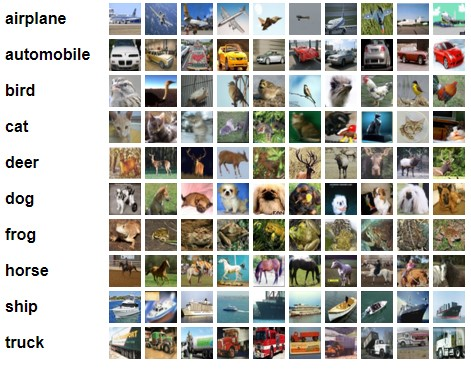
\includegraphics[width=\textwidth, height=5cm, natwidth=1227, natheight=187]{cifar10.jpg}
  \caption{Приклад зображень з датасету CIFAR-10}
  \label{fig:cifar10}
\end{figure}

\subsection{Аналіз роботи алгоритму Deep Infomax}

Робота методу Deep InfoMax буде розглядатись в залежності від значеть гіперпараметрів $\alpha, \, \beta \, \text{та} \, \gamma$, а також коефіціенту швидкості навчання. В кожному експерименті кількість епох навчання нейронної мережі складатиме 300.

Якщо взяти $\alpha = 0,1 \, \beta = 0,1 \, \text{та} \, \gamma = 0,1$, то помилка на тренувальних даних буде 12,73 \% (див. рис. \ref{fig:deepinfoerror1}) та модель тренувалась приблизно 14 годин.

\vspace{1em}

\begin{figure}[h]
  \includegraphics[width=\textwidth, height=7cm, natwidth=854, natheight=476]{deepinfoerror1.jpg}
  \caption{Залежність помилки від епохи навчання при $\alpha = 0,1; \, \beta = 0,1; \, \gamma = 0,1$}
  \label{fig:deepinfoerror1}
\end{figure}

На рис. \ref{fig:deepinfodemo1} можна побачити, що модель доволі погано узагальнює результати.

\vspace{1em}

\begin{figure}[h]
  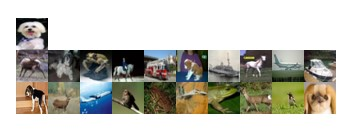
\includegraphics[width=\textwidth, height=7cm, natwidth=854, natheight=476]{deepinfodemo1.jpg}
  \caption{Результати тестування при $\alpha = 0,1; \, \beta = 0,1; \, \gamma = 0,1$}
  \label{fig:deepinfodemo1}
\end{figure}

Якщо взяти $\alpha = 0,5 \, \beta = 0,5 \text{та} \, \gamma = 0,5$, то помилка на тренувальних даних буде 8,05 \% (див. рис. \ref{fig:deepinfoerror2}) та модель тренувалась приблизно 11 годин.

\vspace{1em}

\begin{figure}[h]
  \includegraphics[width=\textwidth, height=7cm, natwidth=854, natheight=476]{deepinfoerror2.jpg}
  \caption{Залежність помилки від епохи навчання при $\alpha = 0,5; \, \beta = 0,5; \, \gamma = 0,5$}
  \label{fig:deepinfoerror1}
\end{figure}

При $\alpha = 0,5 \, \beta = 0,9 \text{та} \, \gamma = 0,1$ помилка на тренувальних даних буде 1,28 \% (див. рис. \ref{fig:deepinfoerror2}) та модель тренувалась приблизно 6 годин.

\vspace{1em}

\begin{figure}[h]
  \includegraphics[width=\textwidth, height=7cm, natwidth=854, natheight=476]{deepinfoerror3.jpg}
  \caption{Залежність помилки від епохи навчання при $\alpha = 0,5; \, \beta = 0,9; \, \gamma = 0,1$}
  \label{fig:deepinfoerror1}
\end{figure}

Якщо взяти $\alpha = 0,5 \, \beta = 1 \text{та} \, \gamma = 0,1$, то помилка на тренувальних даних буде 1,43 \% (див. рис. \ref{fig:deepinfoerror2}) та модель тренувалась приблизно 6 годин.

\vspace{1em}

\begin{figure}[h]
  \includegraphics[width=\textwidth, height=7cm, natwidth=854, natheight=476]{deepinfoerror4.jpg}
  \caption{Залежність помилки від епохи навчання при $\alpha = 0,5; \, \beta = 1; \, \gamma = 0,1$}
  \label{fig:deepinfoerror4}
\end{figure}

Отже, найкращі результати модель отримує при $\alpha = 0,5 \, \beta = 0,9 \text{та} \, \gamma = 0,1$. Результати тестування з даними гіперпараметрами наведено на рис. \ref{fig:deepinfodemo2}.

\vspace{1em}

\begin{figure}[h]
  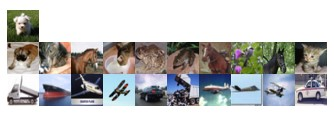
\includegraphics[width=\textwidth, height=7cm, natwidth=854, natheight=476]{deepinfodemo2.jpg}
  \caption{Результати тестування при $\alpha = 0,5; \, \beta = 1; \, \gamma = 0,1$}
  \label{fig:deepinfodemo2}
\end{figure}

Усі вищенаведені результати були отримані з урахуванням коефіціенту швидкості навчання 0,001. Розглянемо результати роботи алгоритму з оптимальними гіперпараметрами з урахуванням інших можливих значень цього коефіціента.

Якщо взяти коефіціент швидості навчання 0,003 то помилка на тренувальних даних буде 1,35 \% (див. рис. \ref{fig:deepinfoerror2}) та модель тренувалась приблизно 6 годин.

\vspace{1em}

\begin{figure}[h]
  \includegraphics[width=\textwidth, height=7cm, natwidth=854, natheight=476]{deepinfoerror5.jpg}
  \caption{Залежність помилки від епохи навчання при коефіціенті швидкості навчання 0,003}
  \label{fig:deepinfoerror5}
\end{figure}



\subsection{Аналіз роботи алгоритму Momentum Contrast}




\subsection{Висновки за розділом}

В даному розділі була продемонстрована робота алгоритмів Deep InfoMax та Momentum Contrast. БУли реалізовані програми мовою програмування Python за допомогою спеціальних бібліотек для аналізу даних та програмного фреймворку Anaconda. 

Як видно з результатів, модель Deep InfoMax дає якісніший прогноз, в той час як алгоритм Momentum Contrast потребує менше часових та обчислювальних ресурсів.
